%-----------------------------------------------------------------
% UNIOESTE - Ciência da Computação
% 4o. ano - Trabalho de Conclusão de Curso
% Profas. Teresinha Arnauts Hachisuca e Izaura
%-----------------------------------------------------------------
%DECLARAÇÃO DO TIPO DE DOCUMENTO, TAMANHO DA FOLHA E FONTE
 %-----------------------------------------------------------------
\documentclass[
    % -- opções da classe memoir --
    12pt,               % tamanho da fonte
%   twoside,            % para impressão em verso e anverso. Oposto a oneside
    a4paper,            % tamanho do papel.
    % -- opções da classe abntex2 --
    %chapter=TITLE,     % títulos de capítulos convertidos em letras maiúsculas
    %section=TITLE,     % títulos de seções convertidos em letras maiúsculas
    %subsection=TITLE,  % títulos de subseções convertidos em letras maiúsculas
    %subsubsection=TITLE,% títulos de subsubseções convertidos em letras maiúsculas
    % -- opções do pacote babel --
    english,            % idioma adicional para hifenização
    brazil,             % o último idioma é o principal do documento
    ]{article}

%-----------------------------------------------------------------
%DEFINIÇÕES DOS PACOTES UTILIZADOS
%-----------------------------------------------------------------
\usepackage{cmap}               % Mapear caracteres especiais no PDF
\usepackage{lmodern}            % Usa a fonte Latin Modern
\usepackage[T1]{fontenc}        % Selecao de codigos de fonte.
\usepackage[utf8]{inputenc}     % Codificacao do documento (conversão automática dos acentos)
\usepackage{lastpage}           % Usado pela Ficha catalográfica
%\usepackage{indentfirst}       % Indenta o primeiro parágrafo de cada seção.
\usepackage{color}              % Controle das cores
\usepackage{graphicx}           % Inclusão de gráficos

\usepackage[brazil]{babel}      % Permite traduzir termos do LateX para português Brasil.
\usepackage{hyperref}           % Permite ativar hyperlinks
\usepackage{algorithm}          % pacote que de suporte a representação de algoritmos.

\usepackage{algorithmic}
\usepackage[pdftex]{geometry}
\usepackage{multirow}
\usepackage{siunitx}

% ---
% Pacotes de citações
% ---
\usepackage[brazilian,hyperpageref]{backref}     % Paginas com as citações na bibl
\usepackage[alf]{abntex2cite}   % Citações padrão ABNT
%\citebrackets[]

% ---
% CONFIGURAÇÕES DE PACOTES
% ---

% ---
% Configurações do pacote backref
% Usado sem a opção hyperpageref de backref
\renewcommand{\backrefpagesname}{Citado na(s) página(s):~}

% Texto padrão antes do número das páginas
\renewcommand{\backref}{}

% Define os textos da citação
\renewcommand*{\backrefalt}[4]{
    \ifcase #1 %
        Nenhuma citação no texto.%
    \or
        Citado na página #2.%
    \else
        Citado #1 vezes nas páginas #2.%
    \fi}%
% ---

%-----------------------------------------------------------------
%               INICIO DO DOCUMENTO - CAPA
%-----------------------------------------------------------------
\begin{document}

\begin{center}

    \textsc{
        \large
            \\universidade estadual do oeste do paraná
            \\unioeste - campus de foz do iguaçu
            \\centro de engenharias e ciências exatas
            \\curso de ciência da computação
            \\[1 cm]tcc - trabalho de conclusão de curso
    }
    \\
    [4 cm]
    \large Proposta de Trabalho de Conclusão de Curso
    \\
    \textbf{
        \textsc{Desenvolvimento de uma Rede de Sensores Sem Fio de Baixo Custo}}
    }
    \\[5 cm]Augusto Lopez Dantas
    \\Orientador: Jorge Habib Hanna El Khouri
    \\[2 cm]Foz do Iguaçu, 23 de julho de 2015

\end{center}

\thispagestyle{empty}

%-----------------------------------------------------------------
%               IDENTIFICAÇÃO DO PROJETO
%-----------------------------------------------------------------
\section{Identificação}

    \subsection{Área e Linha de Pesquisa}
        \noindent Grande Área: Engenharias
        \\Código: 30000009
        \\[1 cm]Linha de Pesquisa: Engenharia Elétrica
        \\Código: 30400007
        \\[1 cm]Especialidade: Automação Eletrônica de Processos Elétricos e Industriais
        \\Código: 30405025

    \subsection{Palavras-chave}

        \begin{enumerate}
            \item Domótica
			\item Rede de Sensores Sem Fio
			\item Comunicação por radiofrequência
        \end{enumerate}


%-----------------------------------------------------------------
%               INTRODUÇÃO E JUSTIFICATIVA
%-----------------------------------------------------------------
\section{Introdução e Justificativa}
Ao longo dos anos, a computação e suas aplicações se tornaram cada vez mais presentes no nosso cotidiano. Uma série de fatores
contribuiu com a rápida difusão da tecnologia em vários setores, como os ambientes domésticos e empresariais, com o objetivo de
melhorar aspectos de controle, eficiência e gestão.

Embora já na década de 60 casas eletricamente sofisticadas eram construídas, foi durante a primeira metade da década de 1980 que o
termo  ``casa inteligente'' passou a ser utilizado, pois o que determina uma casa inteligente não é o quão bem é construída ou
quão efetiva ela é em relação ao espaço, mas sim as tecnologias interativas que ela contém. \cite{harper2003}

Para \citeonline{aldrich2003}, uma casa inteligente pode ser definida como uma residência equipada de tecnologias computacionais
que antecipam e respondem às necessidades dos ocupantes, promovendo conforto, conveniência, segurança e entretenimento através do
gerenciamento da tecnologia interna e conexões com o mundo afora.

Além disso, como a redução de consumo elétrico é um dos principais atrativos em uma casa inteligente, ela normalmente possui
integrações com fontes de energias renováveis, como a solar e a eólica.

O termo domótica origina-se da junção das palavras \textit{domus}, latim para "casa", e robótica, que remete à automação. Sendo
assim, domótica pode ser traduzida como automação residencial, porém, grande parte de seus conceitos também pode ser aplicada a
diversos ambientes como escritórios, indústrias, entre outros.

Segundo \citeonline{riley2012}, domótica é um produto ou serviço que proporciona algum nível de ação ou mensagem para o ambiente
domiciliar, um evento que foi gerado sem a intervenção direta do morador. Um despertador ou um alarme de incêndio são exemplos
disso, porém, esses dispositivos autônomos não necessariamente possuem um mecanismo de comunicação entre eles, limitando o nível
da automação e inteligência da solução.

Sob uma perspectiva técnica, automação residencial consiste em cinco princípios: dispostivos sob controle, que são todos os
eletrodomésticos e eletrônicos de consumo que estão conectados e controlados pelo mesmo sistema de automatização; sensores e
atuadores, que agem como os olhos e mãos da rede residencial medindo e controlando o ambiente; dispositivos de controle remoto,
como um \textit{smartphone}, que possibilitam a interação do usuário com a aplicação; controlador, um sistema computacional que
coleta informações através dos sensores e recebe comandos através do dispositivo de controle remoto; e redes de controle, que
fornecem a comunicação entre as tecnologias envolvidas. \cite{kyas2013}

Em relação à rede de controle, essa pode existir em três formatos: sem fio, com fio ou utilizando cabos energia elétrica. As três
tecnologias têm melhorado significamente em termos de velocidade, confiabilidade e interoperabilidade através da padronização nos
últimos dez anos. \cite{kyas2013}

Contudo, ainda hoje não há um protocolo de comunicação que seja inteiramente adotado, em parte devido ao fato de requerer que os
fabricantes concordem em criar eletrônicos com as mesmas interfaces e protocolos designados em seus produtos. Porém, as tentativas
em padronizar a comunicação na domótica existem desde quase seu início. Uma das primeiras tentativas foi o X10, que utilizava a
rede elétrica existente para transmitir mensagens através de pulsos codificados, mas devido a diversos problemas, como degradação
de sinal e dificuldade para verificação de pacotes, ele acabou não ganhando muita aceitação. \cite{riley2012}

A expectativa é que todos os dispositivos eletroeletrônicos possuam conexão à internet, conceito que vem sendo chamado de Internet
das Coisas e que prevê o endereçamento único para todos os nós conectados na rede mundial através da implantação do IPv6. Este
último é uma evolução do protocolo de rede IPv4 e surgiu em 1994 com a intenção de resolver a limitação de espaço de endereço
prevista e fornecer funcionalidades adicionais. \cite{hagen2002}

Entretanto, a adoção do IPv6 de forma unânime ainda não aconteceu mesmo depois de duas décadas desde sua criação. Além disso, sua
utilização completa em domótica levanta a questão quanto à necessidade em conectar dispositivos simples como sensores e atuadores
à \textit{internet}, levando em consideração custo de implementação e vulnerabilidade. Alternativamente, existe a possibilidade em
desenvolver uma rede específica para esses transdutores, permitindo implementar o monitoramento de um ambiente inteligente de
maneira simples e eficaz.

Essa rede específica, conhecida como rede de sensores [e atuadores], é uma infraestrutura composta por dispositivos de medição e
atuação, de computação e de comunicação que possibilitam instrumentar, observar e reagir à eventos e fenômenos em um determinado
ambiente. \cite{sohraby_minoli_znati2007}

Os quantitativos físicos que podem ser medidos são diversos, como temperatura, umidade, som, luz, radiação, etc. Como
consequência, são várias as possibilidades de aplicação. Algumas das mais comuns são automação residencial e comercial,
monitoramento ambiental e industrial, controle de tráfego, aplicações militares e assistência médica. A complexidade da rede deve
ser proporcial à sua aplicação e vários aspectos devem ser levados em consideração, como por exemplo o meio de comunicação optado.
\cite{kuorilehto2007}

A utilização de fios para realizar tal tarefa é normalmente descartada devido a diversos fatores como custo, manutenção,
localização e mobilidade. Portanto, uma comunicação sem fio, na maioria dos cenários, é um requisito inevitável. Com isso, surgiu
o termo Rede de Sensores Sem Fio (RSSF), que, apesar do nome, frequentemente também inclui atuadores.  \cite{karl_willig2005}

A Figura \ref{figura:wsn} ilustra um sistema de domótica utilizando uma rede sem fio para comunicação apenas com os sensores e
atuadores ao invés de uma única rede de controle entre todos os dispotivos.

\begin{figure}[H]
	\centering
	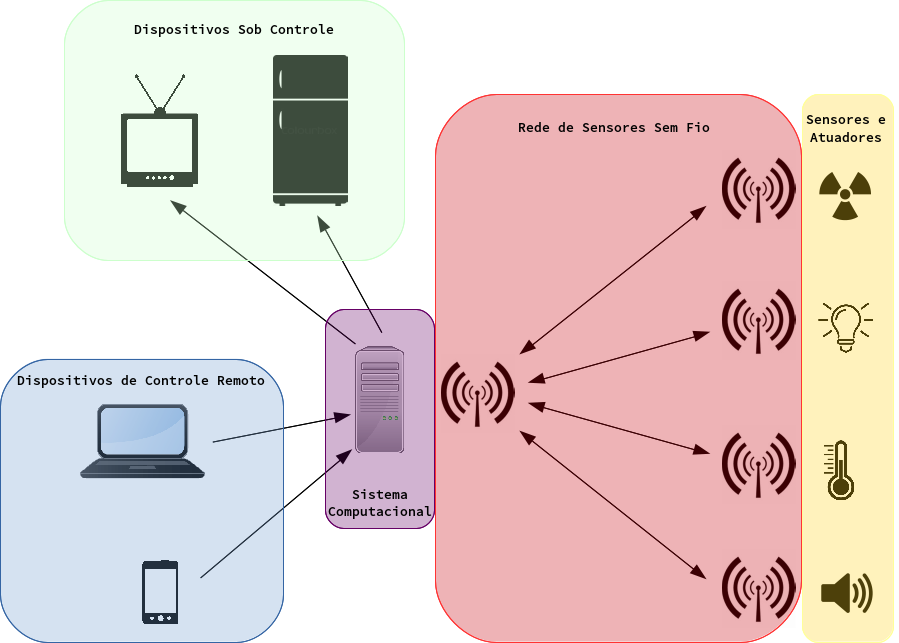
\includegraphics[width=\textwidth]{images/wsn.png}
	\caption{Esboço de uma automação residencial}
	\label{figura:wsn}
\end{figure}

No caso da aplicação deste conceito em domótica, é preferível que a implementação da RSSF seja simples, a fim de obter uma solução
com baixo custo e baixo consumo de eletricidade. Sendo assim, é necessário escolher a tecnologia adequada para tal feito. O
protocolo Wi-Fi, por exemplo, foi taxado como muito complexo e com suporte a largura de banda maior que o necessário; já sistemas
infravermelho requerem uma linha de visão, o que nem sempre é possível neste caso. A tecnologia Bluetooth, por sua vez, aparentou
ser promissora no início mas logo foi julgada como cara e complexa. Isso acabou abrindo as portas para a criação do padrão IEEE
802.15.4 no ano de 2003.  \cite{sohraby_minoli_znati2007}

A tecnologia IEEE 802.15.4 é um sistema de comunicação por rádio frequência de baixo alcance projetado para ter baixa
complexidade, baixo custo, baixo consumo de energia e baixa taxa de transmissão de dados. Esse padrão implementa as camadas física
e de enlace do modelo ISO/OSI e é amplamente utilizado na construção de RSSFs. Além disso, serve como base para outros protocolos
que implementam camadas superiores, como por exemplo o protocolo ZigBee, que fornece mecanismos para entrada e saída em uma rede,
segurança de pacotes, roteamento, descoberta de caminho (para casos de rede malha), entre outros recursos. \cite{buratti2011}

Outro protocolo que se baseia no padrão IEEE 802.15.4 é o 6LoWPAN(\textit{IPv6 over Low power Wireless Personal Area Networks}),
que possibilita o uso eficiente do IPv6 sobre redes sem fio de baixa taxa e baixo consumo de energia em dispositivos embarcados
simples através de uma camada de adaptação e da otimização dos protocolos relacionados. \cite{shelby_bormann2009}

Porém, os módulos que utilizam esses protocolos sofisticados possuem um preço relativamente maior em relação aos módulos com
funcionamento mais básico e acabam inflando o custo total da RSSF de acordo com o número de nós da mesma. Portanto, a fim de se
obter uma solução barata é necessário utilizar um transceptor simples e uma unidade de controle externa de baixo custo para
implementar as demais funcionalidades não realizadas pelo módulo.

Como consequência, ao abrir mão das facilidades que os protocolos de comunicação avançados proporcionam, o esforço requerido para
o desenvolvimento de uma RSSF acaba se tornando maior, sendo necessário definir e implementar diversos aspectos da mesma.

%-----------------------------------------------------------------
%                       OBJETIVO
%-----------------------------------------------------------------
\section{Objetivos}

	%-------------------------------------------------------------------------------

	\subsection{Objetivo Geral}

	Desenvolver uma rede de sensores sem fio, simples e eficáz, para aplicação em automação de residências e escritórios
	utilizando tecnologias existentes e visando baixo custo e baixo consumo elétrico.
	%-------------------------------------------------------------------------------

	\subsection{Objetivos Específicos}

	Os principais objetivos específicos são:

	\begin{itemize}
		\item Rede: definir a topologia, comportamento e roteamento da camada de rede;
		\item Mensagens: definir o escopo das mensagens utilizadas na comunicação;
		\item Biblioteca: desenvolver uma pequena biblioteca com as funcionalidades necessárias para a solulção;
		\item Protótipos: montar protótipos dos pontos de comunicação e realizar a comunicação entre eles.
	\end{itemize}
	%-------------------------------------------------------------------------------


%-----------------------------------------------------------------
%           PLANO DE TRABALHO E CRONOGRAMA DE EXECUÇÃO
%-----------------------------------------------------------------
\section{Plano de Trabalho e Cronograma de Execução}

\begin{enumerate}

	\item Revisão Bibliográfica: elaboração da revisão bibliográfica cujo os principais temas abordados serão:
		\begin{itemize}
			\item Automação;
			\item Domótica;
			\item Sensores e Atuadores;
			\item Comunicação por radiofrequência;
			\item Rede de Sensores sem Fio;
		\end{itemize}

	\item Desenvolvimento:
		\begin{itemize}
			\item Detalhamento dos requisitos do sistema;
			\item Elaboração da arquitetura da solução;
			\item Desenvolvimento e construção da solução;
			\item Testes de verificação e validação dos requisitos.
		\end{itemize}

	\item Monografia: elaboração da monografia do Trabalho de Conclusão de Curso para ser entregue à banca examinadora;

	\item Artigo: elaboração de artigo para submissão em congresso de carácter científico;

	\item Apresentação: apresentação final perante a banca examinadora.

\end{enumerate}

As atividades ocorrerão de acordo com o cronograma apresentado na Tabela \ref{tabela:cronograma}.

\begin{table}[H]
    \scriptsize
    \centering
    \begin{tabular}{|l|c|c|c|c|c|c|c|}
        \hline &  \multicolumn{7}{|c|}
        {\textbf{Período}} \\ \cline{2-8}
        \textbf{Atividades}     &Ago/15      &Set/15      &Out/15      &Nov/15      &Dez/15      &Jan/16      &Fev/16 \\ \hline \hline
        1 - Revisão Bibliográfica  &$\bullet$&$\bullet$&&&&&  \\ \hline
        2 - Desenvolvimento  &&$\bullet$&$\bullet$&$\bullet$&$\bullet$&$\bullet$&  \\ \hline
        3 - Monografia  &&&$\bullet$&$\bullet$&$\bullet$&$\bullet$&  \\ \hline
        4 - Artigo   &&&&&$\bullet$&$\bullet$&  \\ \hline
        5 - Apresentação &&&&&&&$\bullet$&  \hline

    \end{tabular}
     \caption{Cronograma das Atividades}
    \label{tabela:cronograma}
\end{table}

%-----------------------------------------------------------------
%                   MATERIAL E MÉTODO
%-----------------------------------------------------------------

\section{Material e Método}

Os materiais utilizados devem ser compatíveis com o objetivo da solução, ou seja, devem possuir baixo custo e baixo consumo de
energia elétrica. Em relação aos dispositivos de comunicação, existem várias opções com essas características simplistas
disponíveis no mercado.

Uma possibilidade é utilizar o transceptor \texttt{CC2500} da empresa \textit{Texas Instruments}, que implementa o padrão IEEE
802.15.4 e possui uma taxa máxima de transmissão aérea de 500 Kbps, consumindo \SI{17}{\milli \ampere} durante recepção,
\SI{21.2}{\milli \ampere} durante transmissão e \SI{1.5}{\milli \ampere} em modo de espera. Devido ao baixo consumo elétrico e
ótimo custo-benefício, esse dispositivo é amplamente utilizado. \cite{ccdatasheet}

Outro transceptor de rádio frequência bastante difundido é o \texttt{nRF24L01+} da empresa \textit{Nordic Semiconductor}. Embora
possui a desvantagem de não seguir o padrão aberto da IEEE, esse dispositivo apresenta diversas vantagens em relação aos demais
módulos dessa categoria. Uma das principais vantagens é sua taxa máxima de transmissão aérea de 2 Mpbs (quatro vezes mais que o
\texttt{CC2500}) e que, ao mesmo tempo, consome menos energia elétrica que os demais, sendo \SI{13.5}{\milli \ampere} durante
recepção, \SI{11.3}{\milli \ampere} durante transmissão e \SI{26}{\micro \ampere} em modo de espera.  \cite{nrfdatasheet}

Além disso, o \texttt{nRF24L01+} oferece serviços como reconhecimento e retransmissão de pacotes automáticos, diminuindo o número
de comunicação com a unidade microtronladora tal como o processamento utilizado pela mesma. Dessa forma, além de reduzir ainda
mais o consumo elétrico necessário, possibilita uma implementação eficiente utilizando microcontroladores simples e baratos,
tornando-o então, a tecnologia escolhida para a implementação deste trabalho.

Quanto aos microcontroladores, foi optada a utilização dos modelos \texttt{AVR} da empresa \textit{Atmel Corporation}, pois
possuem todas as funcionalidades necessárias para o desenvolvimento do projeto e oferecem \textit{softwares} abertos e gratuitos
para realizar a implementação do código embarcado. Um deles é o compilador \texttt{avr-gcc}, que é uma variação do \textit{GNU
Compiler Collection} e utiliza a biblioteca \texttt{AVR-Libc} que fornece um subconjunto da biblioteca C padrão. Além disso, há
também o programa \texttt{avrdude}, que é o responsável em transferir o código binário gerado para o microcontrolador.

O \textit{software} da solução será desenvolvido em ambiente \texttt{GNU/Linux}, utilizando o \texttt{Vim} como editor de
código-fonte, o \texttt{git} como sistema de controle de versão e o \texttt{make} para auxiliar na compilação e gravação do
projeto. Além disso, serão utilizados vários dispositivos elétricos, como gravador de microcontrolador, \textit{protoboards},
resistores, capacitores, \textit{jumpers}, sensores diversos, LEDs, conversor serial, entre outros.

O projeto será realizado juntamente com pesquisas a materiais de estudo, tal como especificações técnicas das tecnologias
utilizadas. Cada funcionalidade implementada será testada individualmente para garantir uma melhor estabilidade no processo de
escalação da solução.


%-----------------------------------------------------------------
%               CRITÉRIOS DE AVALIAÇÃO
%-----------------------------------------------------------------
\section{Critérios de Avaliação}

Os critérios a serem avaliados são:
\begin{itemize}
	\item Custo e Consumo: o valor monetário necessário para a construção da RSSF, assim como a quantidade de eletricidade
	utilizada pela solução. As informações inferidas através das especificações dos produtos e de lojas revendedoras serão
	comparadas com outras tecnologias similares.
	\item Confiabilidade: levando em consideração quantidade de nós na rede, distância média entre eles e tamanho e integridade de pacotes;
	\item Código-fonte: a organização, legibilidade e funcionalidade do código-fonte.
\end{itemize}

%-----------------------------------------------------------------
%                       REFERÊNCIAS
%-----------------------------------------------------------------

\newpage
\section{Referências}
    \vspace{-4.3em}
    \renewcommand\refname{}
    \bibliography{bibliografia}

%-----------------------------------------------------------------
%                   SÍNTESE BIBLIOGRÁFICA
%-----------------------------------------------------------------
\section{Síntese Bibliográfica}

\bibitem[Atmel Corporation 2009]{avrdatasheet}
\abntrefinfo{Atmel Corporation}{ATMEL CORPORATION}{2009}
{ATMEL CORPORATION. \emph{8-bit AVR Microcontroller with 4/8/16/32K Bytes
  In-System Programmable Flash}.
San Jose, CA, 2009.}

\bibitem[Dargie e Poellabauer 2010]{dargie_poellabauer2010}
\abntrefinfo{Dargie e Poellabauer}{DARGIE; POELLABAUER}{2010}
{DARGIE, W.; POELLABAUER, C. \emph{Fundamentals of wireless sensor networks}.
  Chichester, West Sussex, U.K.: Wiley, 2010.}

\bibitem[Gadre 2001]{gadre2001}
\abntrefinfo{Gadre}{GADRE}{2001}
{GADRE, D.~V. \emph{Programming and customizing the AVR microcontroller}. New
  York: McGraw-Hill, 2001.}

\bibitem[Karl e Willig 2005]{karl_willig2005}
\abntrefinfo{Karl e Willig}{KARL; WILLIG}{2005}
{KARL, H.; WILLIG, A. \emph{Protocols and architectures for wireless sensor
  networks}. Hoboken, NJ: Wiley, 2005.}

\bibitem[L\'opez e Zhou 2008]{lopez_zhou2008}
\abntrefinfo{L\'opez e Zhou}{L\'OPEZ; ZHOU}{2008}
{L\'OPEZ, J.; ZHOU, J. \emph{Wireless sensor network security}. Amsterdam: IOS
  Press, 2008.}

\bibitem[Nordic Semiconductor 2008]{nrfdatasheet}
\abntrefinfo{Nordic Semiconductor}{NORDIC SEMICONDUCTOR}{2008}
{NORDIC SEMICONDUCTOR. \emph{nRF24L01+: Single Chip 2.4GHz Transceiver -
  Product Specification v1.0}.
Trondheim, 2008.}

\bibitem[Trevennor 2012]{trevennor2012}
\abntrefinfo{Trevennor}{TREVENNOR}{2012}
{TREVENNOR, A. \emph{Practical AVR microcontrollers}. Berkeley, CA: Apress,
  2012.}

\bibitem[Williams 2014]{williams2014}
\abntrefinfo{Williams}{WILLIAMS}{2014}
{WILLIAMS, E. \emph{Make: AVR Programming}. Sebastopol, Calif.: Maker Media,
  2014.}

\bibitem[Aldrich 2003]{aldrich2003}
\abntrefinfo{Aldrich}{ALDRICH}{2003}
{ALDRICH, F.~K. Smart homes: Past, present and future. In:  HARPER, R. (Ed.).
  \emph{Inside the Smart Home}. London: Springer, 2003.}

\bibitem[Buratti 2011]{buratti2011}
\abntrefinfo{Buratti}{BURATTI}{2011}
{BURATTI, C. \emph{Sensor networks with IEEE 802.15.4 systems}. Berlin:
  Springer, 2011.}

\bibitem[Hagen 2002]{hagen2002}
\abntrefinfo{Hagen}{HAGEN}{2002}
{HAGEN, S. \emph{IPV6 essentials}. Beijing: O'Reilly, 2002.}

\bibitem[Harper 2003]{harper2003}
\abntrefinfo{Harper}{HARPER}{2003}
{HARPER, R. Inside the smart home: Ideas, possibilities and methods. In:
  HARPER, R. (Ed.). \emph{Inside the Smart Home}. London: Springer, 2003.}

\bibitem[Kuorilehto et al. 2007]{kuorilehto2007}
\abntrefinfo{Kuorilehto et al.}{KUORILEHTO et al.}{2007}
{KUORILEHTO, M. et al. \emph{Ultra-low energy wireless sensor networks in
  practice}. Chichester, England: John Wiley & Sons, 2007.}

\bibitem[Kyas 2013]{kyas2013}
\abntrefinfo{Kyas}{KYAS}{2013}
{KYAS, O. \emph{How To Smart Home}. Wyk, Germany: Key Concept Prees e.K.,
  2013.}

\bibitem[Riley 2012]{riley2012}
\abntrefinfo{Riley}{RILEY}{2012}
{RILEY, M. \emph{Programming your home}. Dallas, Tex.: Pragmatic Bookshelf,
  2012.}

\bibitem[Shelby e Bormann 2009]{shelby_bormann2009}
\abntrefinfo{Shelby e Bormann}{SHELBY; BORMANN}{2009}
{SHELBY, Z.; BORMANN, C. \emph{6LoWPAN: The Wireless Embedded Internet}.
  Chichester, U.K.: J. Wiley, 2009.}

\bibitem[Sohraby, Minoli e Znati 2007]{sohraby_minoli_znati2007}
\abntrefinfo{Sohraby, Minoli e Znati}{SOHRABY; MINOLI; ZNATI}{2007}
{SOHRABY, K.; MINOLI, D.; ZNATI, T.~F. \emph{Wireless sensor networks}.
  Hoboken, N.J.: Wiley-Interscience, 2007.}

\bibitem[Texas Instruments 2015]{ccdatasheet}
\abntrefinfo{Texas Instruments}{TEXAS INSTRUMENTS}{2015}
{TEXAS INSTRUMENTS. \emph{CC2500 - Low-Cost Low-Power 2.4 GHz RF Transceiver}.
Dallas, Texas, 2015.}




\end{document}
